% =============================================================================
%  Rapport d'ingénierie des données — Projet 1 : indicateurs ODD 3 de l'OMS (FR)
%  Compilation : latexmk -xelatex rapport-fr.tex   (voir README.md de ce dossier)
% =============================================================================
\documentclass[11pt, a4paper, oneside, headings=normal, numbers=noenddot, DIV=12]{scrartcl}
\usepackage[french]{babel}
\usepackage{report-style}
\graphicspath{{../livraison/figures/fr/}}
\sisetup{locale=FR, group-minimum-digits=4}

% --- Résultats de la recette (renseignés après exécution sur environnement neuf) ---
\newcommand{\RecInstall}{57~s}
\newcommand{\RecPipeline}{2~min~43~s (extraction réelle comprise)}
\newcommand{\RecRows}{\num{129368}}

% --- Métadonnées ---------------------------------------------------------------
\newcommand{\ReportAuthor}{LUMU BAMANA MANASSE}
\newcommand{\ReportAuthorRole}{Data engineer}
\newcommand{\ReportShortTitle}{Indicateurs ODD 3 de l'OMS · Rapport d'ingénierie des données}
\newcommand{\ReportFooter}{Octobre 2026 · v1.0.0}
\newcommand{\ReportKicker}{Rapport d'ingénierie des données · Projet 1}
\newcommand{\ReportTitle}{Santé mondiale :\\les ODD 3 en Afrique}
\newcommand{\ReportSubtitle}{Un entrepôt PostgreSQL fiable des indicateurs de l'OMS :\\ingestion, qualité, UPSERT et analyse des cibles 2030}
\newcommand{\ReportMeta}{%
  \begin{tabularx}{\linewidth}{@{}>{\bfseries}l@{\hspace{1em}}Y@{}}
  Date & Octobre 2026 \\
  Version & 1.0.0 (livrée et recettée) \\
  Client & Initiative Baobab Santé (ONG fictive) · Mission IBS-2026-001 \\
  Dépôt GitHub & \url{https://github.com/MediJr/who-sdg3-health-etl} \\
  Langue & Français · \textit{English version available in the repository}
  \end{tabularx}}
\newcommand{\ReportScenario}{Scénario fictif, données réelles : l'ONG cliente et ses interlocuteurs sont inventés pour simuler une mission
  professionnelle complète. Les données proviennent de l'Observatoire mondial de la santé de l'OMS (Global Health Observatory), extraites
  le 22 octobre 2026. Ce projet n'est ni commandé, ni validé, ni affilié à l'Organisation mondiale de la santé.}
\hypersetup{pdftitle={Santé mondiale : les ODD 3 en Afrique, rapport d'ingénierie des données}, pdfauthor={Lumu Bamana Manasse},
  pdfsubject={Pipeline ETL OMS vers PostgreSQL, projet de portfolio}, pdflang={fr-FR}}

\begin{document}
\MakeTitlePage

% =============================================================================
\section*{Fiche du document}
\addcontentsline{toc}{section}{Fiche du document}

\begin{tabularx}{\linewidth}{@{}>{\bfseries\sffamily}L{4.2cm}Y@{}}
\toprule
Projet & Projet 1 du portfolio : entrepôt PostgreSQL des indicateurs de santé de l'OMS \\
Mission & IBS-2026-001 : « Suivre l'ODD 3 en Afrique avec les données de l'OMS » \\
Client & Initiative Baobab Santé, ONG de santé maternelle et infantile (fictive), à l'attention de Dr Mariam Koné \\
Auteur & Lumu Bamana Manasse, data engineer \\
Période de réalisation & Octobre 2026 \\
Données & API GHO de l'OMS, lot du 22 octobre 2026 \\
Statut & \pill{good}{LIVRÉ} \pill{good}{RECETTÉ} \\
Code source & \url{https://github.com/MediJr/who-sdg3-health-etl} \\
\bottomrule
\end{tabularx}

\subsection*{Historique des versions}
\begin{tabularx}{\linewidth}{@{}l l Y@{}}
\toprule
\textbf{Version} & \textbf{Date} & \textbf{Objet} \\
\midrule
0.1 & 22/10/2026 & Cadrage : brief, compte rendu, cahier des charges \\
0.9 & 22/10/2026 & Pipeline, tests, analyses, corrections (qualité, performance) \\
1.0.0 & 22/10/2026 & Recette sur environnement neuf, rapport final (français et anglais) \\
\bottomrule
\end{tabularx}

\subsection*{Guide de lecture}
\begin{tabularx}{\linewidth}{@{}>{\bfseries}L{4.2cm}Y@{}}
Conseil d'administration & \hyperref[sec:resume]{1. Résumé exécutif} et \hyperref[sec:resultats]{11. Résultats et recommandations} \\
Responsable suivi-évaluation & 2. Cadrage, 6. Modèle de données, 7. Qualité, 12. Limites \\
Ingénieur reprenant le projet & 4. Architecture, 5. Pipeline, 9. Exploitation, 10. Tests, annexes \\
\end{tabularx}

\begingroup
\addtokomafont{sectionentry}{\color{primary}}
\setcounter{tocdepth}{2}
\tableofcontents
\endgroup
\clearpage

% =============================================================================
\section{Résumé exécutif}\label{sec:resume}

\textbf{Le besoin.} L'ONG Initiative Baobab Santé suit chaque année la progression des pays africains vers les cibles de l'ODD 3.
Son processus était manuel (téléchargements, copier-coller dans Excel), non reproductible, et avait déjà produit une erreur présentée
au conseil d'administration : un tableau mélangeait plusieurs catégories de données sans que personne ne le voie.

\textbf{La solution.} Un pipeline Python alimente automatiquement un entrepôt \textbf{PostgreSQL} conteneurisé avec 9 indicateurs
de l'OMS. Le grain est explicite, les contrôles de qualité mettent en quarantaine les lignes invalides, et un chargement
\textbf{UPSERT} intègre les révisions de l'OMS sans jamais créer de doublon. L'équipe du client interroge la base en SQL.

\kpirow{129\,368}{observations\\de l'OMS}{9}{indicateurs\\ODD 3}{386}{lieux (pays,\\régions, monde)}{22 / 22}{tests\\automatisés}
\kpirow{0 / 0}{insertions / mises à jour\\à la relance}{10 s}{rechargement\\complet}{×15}{gain de performance\\après diagnostic}{0}{donnée\\personnelle}

\begin{keybox}[Principaux résultats pour la région africaine de l'OMS (47 pays)]
\begin{itemize}[leftmargin=1.2em]
  \item \textbf{Q1 · Cibles 2030 :} seuls \textbf{5 pays} sur 47 ont atteint la cible de mortalité des moins de 5 ans (25 ‰),
        et 4 celle de la mortalité maternelle (70 pour 100\,000). La région reste loin derrière la moyenne mondiale.
  \item \textbf{Q2 · Rythme :} \textbf{aucun} pays hors cible n'est en voie d'atteindre l'objectif de mortalité infantile d'ici 2030.
        Le pays médian progresse de 3,0~\% par an, alors qu'il lui faudrait 12,4~\% : \textbf{quatre fois plus vite}.
  \item \textbf{Q3 · Inégalités :} un enfant des 20~\% de ménages les plus pauvres a \textbf{1,7 fois plus de risque} de mourir
        avant 5 ans (jusqu'à 2,5 fois au Nigeria). L'écart absolu se réduit, mais l'écart relatif se creuse depuis 2000.
  \item \textbf{Q4 · Moyens :} les \textbf{accouchements assistés} sont le moyen le plus lié à une faible mortalité (corrélation de $-0{,}75$).
\end{itemize}
\end{keybox}

\textbf{Ce que démontre ce projet, côté ingénierie :} conteneurisation d'une base PostgreSQL, gestion des secrets hors du code, modèle
en couches (staging, core, ops), clé métier complète avec \texttt{NULLS NOT DISTINCT}, chargement en masse par \texttt{COPY} suivi d'un UPSERT
idempotent et mesurable, contrôles de qualité avec quarantaine, journal des exécutions, tests unitaires et d'intégration, et deux diagnostics
de production : une panne de Docker et une connexion de 130~secondes ramenée à zéro.

% =============================================================================
\section{Contexte et cadrage}

\subsection{Les vrais problèmes du client}
L'analyse du brief a montré que le problème du client était d'abord un problème d'\textbf{ingénierie des données}, et seulement ensuite d'analyse :

\begin{table}[H]
\centering\small
\begin{tabularx}{\linewidth}{@{}L{4.4cm} Y@{}}
\toprule
\textbf{Symptôme décrit par le client} & \textbf{Cause technique} \\
\midrule
« Nous téléchargeons les tableaux à la main » & Aucun processus reproductible ni traçable \\
« Les chiffres ne concordent jamais d'une année sur l'autre » & L'OMS révise ses estimations, et personne ne garde la trace des révisions \\
« Un tableau mélangeait plusieurs catégories » & \textbf{Erreur de grain} : une même valeur pays-année existe par sexe, par âge et par quintile de richesse \\
\bottomrule
\end{tabularx}
\caption{Du symptôme à la cause}
\end{table}

\subsection{Questions business}
\begin{table}[H]
\centering
\begin{tabularx}{\linewidth}{@{}l Y L{4.2cm}@{}}
\toprule
\textbf{\#} & \textbf{Question} & \textbf{Décision éclairée} \\
\midrule
Q1 & Où en sont les pays de la région africaine par rapport aux cibles ODD 3 de 2030 ? & Diagnostic présenté au conseil \\
Q2 & À leur rythme actuel, quels pays atteindront ces cibles d'ici 2030 ? & Priorisation des pays à financer \\
Q3 & Quel est l'écart de mortalité infantile entre les ménages les plus pauvres et les plus riches ? & Ciblage des programmes \\
Q4 & Les moyens du système de santé vont-ils de pair avec de meilleurs résultats ? & Choix des leviers d'action \\
\bottomrule
\end{tabularx}
\caption{Questions retenues lors du cadrage}
\end{table}

\subsection{Exigences techniques}
\begin{table}[H]
\centering\small
\begin{tabularx}{\linewidth}{@{}L{5.6cm} Y@{}}
\toprule
\textbf{Exigence} & \textbf{Réponse technique} \\
\midrule
Base accessible en SQL à plusieurs utilisateurs & PostgreSQL 17 dans Docker \\
Relançable à tout moment, sans doublon & UPSERT sur une clé métier complète \\
Dernière valeur publiée, et date de révision & \texttt{last\_changed\_at}, \texttt{last\_run\_id} \\
Grain explicite & Clé \texttt{UNIQUE NULLS NOT DISTINCT} sur 7 colonnes \\
Contrôles avant chargement & 9 règles et une table de quarantaine \\
Mots de passe hors du code & Fichier \texttt{.env} exclu de Git \\
Tests automatisés & \texttt{pytest} : 17 tests unitaires et 5 tests d'intégration \\
\bottomrule
\end{tabularx}
\caption{Exigences du cahier des charges et réponses apportées}
\end{table}

\subsection{Périmètre}
La base contient les 9 indicateurs pour \textbf{tous les pays et toutes les régions} publiés par l'OMS : elle est réutilisable au-delà de
cette mission. Les analyses portent sur la \textbf{région africaine de l'OMS} (47 pays avec données), avec la valeur mondiale comme référence.

% =============================================================================
\section{Sources de données}

\begin{table}[H]
\centering\small
\begin{tabularx}{\linewidth}{@{}L{3.4cm} Y L{3.6cm}@{}}
\toprule
\textbf{Ressource GHO} & \textbf{Contenu} & \textbf{Volume (lot du 22/10)} \\
\midrule
\texttt{/api/\{indicateur\}} & Observations : valeur, bornes d'incertitude, date de mise à jour & \num{129368} lignes, 9 indicateurs \\
\texttt{/api/Indicator} & Libellés officiels des indicateurs & 9 lignes \\
\texttt{/api/DIMENSION/}\allowbreak\texttt{\{type\}/}\allowbreak\texttt{DimensionValues} & Libellés des lieux et des ventilations & 386 lieux, 174 ventilations \\
\bottomrule
\end{tabularx}
\caption{Ressources de l'API de l'OMS utilisées (protocole OData, sans clé d'API)}
\end{table}

\begin{table}[H]
\centering\small
\begin{tabularx}{\linewidth}{@{}l Y r l@{}}
\toprule
\textbf{Code} & \textbf{Indicateur} & \textbf{Lignes} & \textbf{Cible 2030} \\
\midrule
\texttt{MDG\_0000000007} & Mortalité des moins de 5 ans (‰) & \num{64510} & $\leq 25$ \\
\texttt{WHOSIS\_000001} & Espérance de vie à la naissance & \num{14112} & – \\
\texttt{WHOSIS\_000002} & Espérance de vie en bonne santé & \num{14112} & – \\
\texttt{WHOSIS\_000003} & Mortalité néonatale (‰) & \num{12128} & $\leq 12$ \\
\texttt{MDG\_0000000026} & Mortalité maternelle (pour 100\,000) & \num{7878} & $< 70$ \\
\texttt{WHS4\_100} & Couverture vaccinale DTP3 (\%) & \num{5337} & 90 \% \\
\texttt{GHED\_CHE\_pc\_US\_SHA2011} & Dépenses de santé par habitant (USD) & \num{4849} & – \\
\texttt{HWF\_0001} & Médecins pour 10\,000 habitants & \num{3693} & – \\
\texttt{MDG\_0000000025} & Accouchements assistés (\%) & \num{2749} & – \\
\bottomrule
\end{tabularx}
\caption{Indicateurs collectés}
\end{table}

\begin{keybox}[Découverte clé de l'exploration : la dimension cachée]
Pour le Sénégal en 2020, la mortalité des moins de 5 ans apparaît \textbf{8 fois avec 8 valeurs différentes}, de 27,9 à 61,2~‰.
Ce ne sont pas des doublons : la colonne \texttt{Dim3} porte le \textbf{quintile de richesse} (61~‰ chez les 20~\% de ménages les plus
pauvres, 28~‰ chez les 20~\% les plus riches). C'est exactement l'erreur commise par le client l'année précédente. Cette découverte a fixé
le \textbf{grain} de la table de faits et a fait naître la question Q3.
\end{keybox}

% =============================================================================
\section{Architecture de la solution}

\begin{figure}[H]
\centering
\resizebox{\linewidth}{!}{%
\begin{tikzpicture}[
  font=\sffamily\small, node distance=0.6cm and 0.8cm,
  src/.style={draw=rule, fill=panel, rounded corners=2pt, minimum width=2.4cm, minimum height=1.2cm, align=center},
  stage/.style={draw=primary, fill=primary, text=white, rounded corners=3pt, minimum width=2.4cm, minimum height=1.2cm, align=center, font=\sffamily\small\bfseries},
  store/.style={cylinder, shape border rotate=90, aspect=0.18, draw=accent, fill=accent!8, minimum width=2.2cm, minimum height=1.4cm, align=center},
  bad/.style={cylinder, shape border rotate=90, aspect=0.18, draw=warn, fill=warn!8, minimum width=2.2cm, minimum height=1.2cm, align=center},
  deliv/.style={draw=accent, rounded corners=2pt, minimum width=2.4cm, minimum height=0.7cm, align=center},
  arr/.style={-{Stealth[length=2.6mm]}, thick, color=ink2}]
  \node[src] (api) {API OMS\\\scriptsize GHO (OData)};
  \node[stage, right=of api] (e) {EXTRACT\\\scriptsize\mdseries réessais · gzip · SHA-256};
  \node[store, below=0.9cm of e] (raw) {\scriptsize data/raw/\\\scriptsize AAAA-MM-JJ};
  \node[stage, right=of e] (t) {TRANSFORM\\\scriptsize\mdseries grain · 9 contrôles};
  \node[bad, above=0.7cm of t] (q) {\scriptsize ops.\\\scriptsize quarantine};
  \node[stage, right=1.5cm of t] (l) {LOAD\\\scriptsize\mdseries COPY → UPSERT};
  \node[store, right=of l, minimum height=1.9cm] (db) {\scriptsize PostgreSQL 17\\\scriptsize staging · core · ops\\\scriptsize (Docker)};
  \node[deliv, right=0.9cm of db, yshift=0.9cm] (o1) {Vues SQL};
  \node[deliv, below=0.25cm of o1] (o2) {Équipe client};
  \node[deliv, below=0.25cm of o2] (o3) {Rapport};
  \draw[arr] (api) -- (e);
  \draw[arr] (e) -- (raw);
  \draw[arr] (raw.east) -| (t.south);
  \draw[arr] (t) -- node[right, font=\scriptsize\sffamily, text=warn]{invalide} (q);
  \draw[arr] (t) -- node[above, font=\scriptsize\sffamily, text=ink2]{valide} (l);
  \draw[arr] (l) -- (db);
  \foreach \o in {o1,o2,o3} \draw[arr] (db.east) -- (\o.west);
  \begin{scope}[on background layer]
    \node[draw=rule, dashed, rounded corners=6pt, fit=(e)(t)(l)(raw)(q), inner sep=9pt, label={[font=\scriptsize\sffamily, text=ink2]above:python -m src.pipeline}] {};
  \end{scope}
\end{tikzpicture}}
\caption{Architecture : une commande collecte, contrôle et charge les données dans PostgreSQL}
\end{figure}

\subsection{Choix techniques}
\begin{table}[H]
\centering\small
\begin{tabularx}{\linewidth}{@{}L{2.6cm} L{3.2cm} Y@{}}
\toprule
\textbf{Besoin} & \textbf{Choix} & \textbf{Justification} \\
\midrule
Base de données & PostgreSQL 17 & Multi-utilisateur, contraintes fortes, UPSERT natif, \texttt{NULLS NOT DISTINCT} (ADR 001) \\
Exécution de la base & Docker Compose & Même base sur tous les postes, en une commande, sans installation manuelle \\
Pilote & psycopg 3 & Pilote moderne, \texttt{COPY} pour le chargement en masse \\
Secrets & python-dotenv + \texttt{.env} & Aucun mot de passe dans le code ni dans Git \\
Réessais HTTP & \texttt{urllib3.Retry} & Attente croissante, respect de l'en-tête \texttt{Retry-After} \\
Tests & pytest & Tests unitaires sans base, tests d'intégration sur une base dédiée \\
\bottomrule
\end{tabularx}
\caption{Stack technique (en plus de Python, pandas et matplotlib, déjà utilisés au projet 0)}
\end{table}

\subsection{Ce qui change par rapport au projet 0}
\begin{table}[H]
\centering\small
\begin{tabularx}{\linewidth}{@{}L{3.2cm} Y Y@{}}
\toprule
& \textbf{Projet 0} & \textbf{Projet 1} \\
\midrule
Base & DuckDB (fichier) & PostgreSQL (serveur, conteneur) \\
Chargement & Rechargement complet & Staging + UPSERT, données conservées \\
Idempotence & Garantie par le remplacement & \textbf{Mesurée} : compteurs insérées / mises à jour / inchangées \\
Qualité & Contrôles a posteriori & Contrôles \textbf{avant} chargement, et quarantaine \\
Secrets & Aucun & Fichier \texttt{.env} \\
Tests & Recette manuelle & 22 tests automatisés \\
Traçabilité & Manifeste & Manifeste avec SHA-256, et journal des exécutions en base \\
\bottomrule
\end{tabularx}
\caption{Progression du portfolio}
\end{table}

% =============================================================================
\section{Conception du pipeline}

\subsection{Extraction}
\begin{itemize}[leftmargin=1.2em]
  \item \textbf{Réessais confiés à \texttt{urllib3.Retry}} : jusqu'à 4 tentatives, avec des attentes de 2, 4, 8 et 16~s, sur les erreurs
        temporaires uniquement (429, 500, 502, 503, 504) et jamais sur une erreur 404.
  \item \textbf{Pagination OData suivie} (\texttt{@odata.nextLink}), et \textbf{échec explicite} si la réponse ne contient pas la clé
        \texttt{value} : mieux vaut planter que charger n'importe quoi.
  \item \textbf{Couche brute compressée} (gzip, 6,4~Mo pour \num{129368} lignes) et \textbf{écriture atomique}.
  \item \textbf{Manifeste} avec l'empreinte SHA-256 de chaque fichier, qui prouve l'intégrité du lot.
\end{itemize}

\subsection{Transformation et contrôles de qualité}
Les ventilations sont rangées selon leur \textbf{type déclaré} (\texttt{Dim1Type}, \texttt{Dim2Type}…), jamais selon leur position :
l'OMS peut placer le sexe en première ou en deuxième dimension selon l'indicateur. Neuf règles sont ensuite appliquées :

\begin{table}[H]
\centering\small
\begin{tabularx}{\linewidth}{@{}l Y@{}}
\toprule
\textbf{\#} & \textbf{Règle (motif de quarantaine)} \\
\midrule
1 & Indicateur hors référentiel \\
2 & Valeur absente ou non numérique \\
3 & Valeur hors bornes de vraisemblance (limites logiques, voir section 7) \\
4 & Intervalle d'incertitude incohérent (borne basse > valeur, ou valeur > borne haute) \\
5 & Année invalide \\
6 & Lieu absent du référentiel \\
7 & Ventilation absente du référentiel \\
8 & Type de ventilation inconnu \\
9 & Doublon de clé métier dans le lot \\
\bottomrule
\end{tabularx}
\caption{Règles de qualité appliquées avant chargement}
\end{table}

\subsection{Chargement : staging et UPSERT}
Le lot est copié en masse dans \texttt{staging.}\allowbreak\texttt{observation} (\texttt{COPY}, 0,9~s), puis fusionné dans \texttt{core.}\allowbreak\texttt{fact\_observation} par
une seule requête :

\begin{lstlisting}[language=DuckSQL]
INSERT INTO core.fact_observation AS f (...)
SELECT ... FROM staging.observation
ON CONFLICT ON CONSTRAINT uq_observation_business_key DO UPDATE SET
    value = EXCLUDED.value, value_low = EXCLUDED.value_low, value_high = EXCLUDED.value_high,
    last_changed_at = now(), last_run_id = EXCLUDED.last_run_id
WHERE (f.value, f.value_low, f.value_high)
      IS DISTINCT FROM (EXCLUDED.value, EXCLUDED.value_low, EXCLUDED.value_high)
RETURNING (xmax = 0) AS inserted      -- vrai : insérée, faux : mise à jour
\end{lstlisting}

\begin{itemize}[leftmargin=1.2em]
  \item \texttt{ON CONFLICT} : si la clé métier existe déjà, on met à jour au lieu d'insérer.
  \item \texttt{WHERE … IS DISTINCT FROM} : on ne touche \textbf{que} les valeurs réellement révisées par l'OMS.
  \item \texttt{IS DISTINCT FROM} plutôt que \texttt{<>} : il compare correctement les \texttt{NULL}, ce que \texttt{<>} ne fait pas.
  \item Fusion, quarantaine et journal sont validés dans \textbf{une seule transaction}. Le journal des exécutions est ouvert à part,
        pour qu'un échec reste tracé.
\end{itemize}

% =============================================================================
\section{Modèle de données}

\begin{figure}[H]
\centering
\resizebox{0.97\linewidth}{!}{%
\begin{tikzpicture}[font=\sffamily\scriptsize,
  ent/.style={draw=primary, fill=white, rounded corners=2pt, align=left, inner sep=5pt},
  ops/.style={draw=ink2, dashed, fill=white, rounded corners=2pt, align=left, inner sep=5pt},
  rel/.style={-{Stealth[length=2mm]}, thick, color=accent}]
  \node[ent, minimum width=5.2cm] (f) {\textbf{\normalsize core.fact\_observation}\\[2pt]
     \textbf{clé métier :} indicator\_code, location\_type, location\_code,\\year, sex, age\_group, wealth\_quintile\\[2pt]
     value, value\_low, value\_high, who\_updated\_at\\first\_loaded\_at, last\_changed\_at, last\_run\_id};
  \node[ent, above left=0.6cm and 0.4cm of f] (i) {\textbf{\normalsize dim\_indicator}\\\textbf{indicator\_code}\\name\_fr, unit, role\\target\_2030, target\_direction};
  \node[ent, above right=0.6cm and 0.4cm of f] (l) {\textbf{\normalsize dim\_location}\\\textbf{location\_type, location\_code}\\name, who\_region};
  \node[ent, below left=0.6cm and 0.4cm of f] (b) {\textbf{\normalsize dim\_breakdown}\\\textbf{breakdown\_code}\\breakdown\_type, label};
  \node[ops, below right=0.6cm and 0.4cm of f] (r) {\textbf{\normalsize ops.pipeline\_run}\\\textbf{run\_id}\\rows\_inserted / updated\\unchanged / quarantined};
  \node[ops, right=0.6cm of r] (q) {\textbf{\normalsize ops.quarantine}\\run\_id, reason\\raw\_record (JSON)};
  \draw[rel] (f) -- (i); \draw[rel] (f) -- (l); \draw[rel] (f) -- node[left, font=\scriptsize]{×3} (b); \draw[rel] (f) -- (r); \draw[rel] (q) -- (r);
\end{tikzpicture}}
\caption{Modèle de données (schémas core et ops ; les flèches représentent les clés étrangères)}
\end{figure}

\begin{keybox}[Pourquoi NULLS NOT DISTINCT ?]
Par défaut, en SQL, \texttt{NULL = NULL} n'est pas vrai : deux lignes « sans ventilation » ne sont donc pas considérées comme des doublons,
et une contrainte d'unicité classique laisserait passer une infinité de copies. \texttt{UNIQUE NULLS NOT DISTINCT} (PostgreSQL 15 et plus)
traite les \texttt{NULL} comme égaux, et ferme cette faille.
\end{keybox}

\textbf{Vues d'analyse.} \texttt{core.v\_national} encapsule la règle de grain (deux sexes, sans ventilation par richesse) et
\texttt{core.v\_latest} donne la dernière année disponible. L'équipe du client n'a plus à connaître ces règles pour obtenir une valeur juste.

% =============================================================================
\section{Qualité des données}

\subsection{Couverture}
Les 9 indicateurs sont disponibles pour les \textbf{47 pays} de la région africaine ayant des données (sur 50 codes de pays et territoires).
Les données sont récentes : 2023 à 2025 selon les indicateurs. Seule exception : les accouchements assistés, pour lesquels seuls 32 pays ont
une donnée postérieure à 2020 (médiane : 2021).

\subsection{Calibrage des seuils : une leçon sur les données réelles}
Au premier passage, des seuils de vraisemblance « intuitifs » ont mis \textbf{25 lignes en quarantaine}. Leur examen a montré qu'il ne s'agissait
pas d'erreurs, mais des traces chiffrées de crises humanitaires majeures :

\begin{table}[H]
\centering\small
\begin{tabularx}{\linewidth}{@{}L{4.6cm} r Y@{}}
\toprule
\textbf{Seuil initial} & \textbf{Lignes} & \textbf{Ce qu'étaient ces valeurs} \\
\midrule
Mortalité des moins de 5 ans ≤ 500~‰ & 18 & Cambodge 1975-1978 (régime khmer rouge), Soudan du Sud 1988, Irak 1942-1944 \\
Mortalité maternelle ≤ \num{5000} & 7 & Rwanda 1994 (génocide), Soudan du Sud 1987-1998 (guerre civile) \\
\bottomrule
\end{tabularx}
\caption{Valeurs extrêmes mais réelles, mises en quarantaine à tort}
\end{table}

Les seuils ont été remplacés par des \textbf{limites logiques} : un taux pour 1\,000 naissances ne dépasse pas 1\,000, un pourcentage pas 100
(ADR 003). Résultat : \textbf{\num{129368} lignes valides, 0 en quarantaine}, et les contrôles continuent de bloquer les erreurs réelles,
comme le prouvent les tests.

\begin{keybox}[Leçon]
Une règle de qualité se calibre avec la connaissance du domaine. La quarantaine a joué son rôle : isoler les valeurs suspectes pour
qu'un humain les examine, au lieu de les supprimer en silence ou de les charger sans examen.
\end{keybox}

% =============================================================================
\section{Sécurité et gouvernance}

\begin{tabularx}{\linewidth}{@{}L{3.6cm} Y@{}}
\toprule
\textbf{Thème} & \textbf{Mesure} \\
\midrule
Secrets & Identifiants PostgreSQL dans \texttt{.env} (exclu de Git). Modèle sans secret \texttt{.env.example} versionné. Mot de passe aléatoire généré localement. \\
Exposition réseau & Base accessible uniquement depuis la machine locale (\texttt{127.0.0.1:5433}) \\
Données personnelles & Aucune : les données de l'OMS sont agrégées à l'échelle des pays \\
Licence des données & Données de l'OMS utilisées selon sa politique d'utilisation des données, à des fins non commerciales, avec mention de la source \\
Traçabilité & Manifeste SHA-256, journal \texttt{ops.pipeline\_run}, \texttt{last\_run\_id} sur chaque observation, ADR, journal de bord \\
\bottomrule
\end{tabularx}

% =============================================================================
\section{Exploitation}

\subsection{Commandes}
\begin{lstlisting}[language=bash]
copy .env.example .env                         # puis choisir un mot de passe
docker compose up -d                           # démarre PostgreSQL (port 5433)
pip install -r requirements.txt
python -m src.pipeline                         # extraction + chargement + rapport
python -m src.pipeline --run-date 2026-10-22   # rejoue un lot brut, sans appel à l'API
pytest                                         # 22 tests (dont 5 sur une base dédiée)
\end{lstlisting}

\subsection{Diagnostics de production}
Deux incidents réels ont été diagnostiqués et résolus pendant la mission :

\begin{table}[H]
\centering\small
\begin{tabularx}{\linewidth}{@{}L{3cm} Y Y@{}}
\toprule
\textbf{Incident} & \textbf{Diagnostic} & \textbf{Résolution} \\
\midrule
Docker Desktop plante au démarrage & Journal du backend : deux sockets Unix (\texttt{sailor-ingest.sock}, \texttt{engine.sock}) verrouillés depuis un arrêt brutal, un mois plus tôt & Dossiers renommés (rien supprimé). Docker recrée des dossiers propres. \\
\midrule
Chargement en 156~s pour \num{129368} lignes & Mesure étape par étape : \texttt{COPY} 0,9~s, UPSERT 2,8~s, mais \textbf{connexion 130~s}. \texttt{localhost} est résolu d'abord en IPv6 (\texttt{::1}), où Docker n'écoute pas. & Hôte \texttt{127.0.0.1} et \texttt{connect\_timeout=10} : pipeline en \textbf{10~s} (×15) \\
\bottomrule
\end{tabularx}
\caption{Incidents résolus}
\end{table}

\begin{keybox}[Leçon]
Mesurer au lieu de supposer : le goulot d'étranglement n'était ni dans le code Python ni dans PostgreSQL, mais dans la résolution du nom d'hôte.
\end{keybox}

% =============================================================================
\section{Tests et recette}

\subsection{Tests automatisés}
\begin{table}[H]
\centering\small
\begin{tabularx}{\linewidth}{@{}L{4.3cm} r Y@{}}
\toprule
\textbf{Fichier} & \textbf{Tests} & \textbf{Ce qui est vérifié} \\
\midrule
\texttt{test\_extract.py} & 4 & Pagination OData, échec sur structure inattendue, écriture atomique, réessais limités aux erreurs temporaires \\
\texttt{test\_transform.py} & 13 & Grain (quintiles distincts), ventilations rangées par type, chacune des règles de quarantaine, aucune ligne perdue \\
\texttt{test\_load\_integration.py} & 5 & Sur une vraie base dédiée : premier chargement, relance idempotente, révision détectée, quarantaine en base, contrainte d'unicité \\
\bottomrule
\end{tabularx}
\caption{22 tests, sur un extrait réel de l'API (Sénégal, 2020)}
\end{table}

Les tests ont trouvé un \textbf{vrai bug} : dans une colonne pandas mixte, \texttt{None} devient \texttt{NaN}, et \texttt{NaN} est « vrai »
en Python. Une seule ligne à la ventilation inconnue envoyait alors \textbf{toutes} les lignes en quarantaine.

\subsection{Recette sur environnement neuf}
Copie des seuls fichiers publiables, nouvel environnement Python, \texttt{.env} recréé à partir du modèle, \textbf{base PostgreSQL vierge},
extraction réelle depuis l'API.

\begin{table}[H]
\centering\small
\begin{tabularx}{\linewidth}{@{}l L{4.6cm} Y c@{}}
\toprule
\textbf{\#} & \textbf{Critère} & \textbf{Résultat} & \\
\midrule
C1 & Exécution de bout en bout, base comprise & Installation en \RecInstall, pipeline en \RecPipeline & \ok \\
C2 & Relance sans doublon ni modification & 0 insérée, 0 mise à jour, \RecRows{} inchangées & \ok \\
C3 & Clé métier couvrant toutes les dimensions & Contrainte en base, 0 doublon, test d'intégration & \ok \\
C4 & Lignes invalides en quarantaine, jamais perdues & Invariant extraites = chargées + quarantaine & \ok \\
C5 & Aucun secret dans le dépôt & \texttt{.env} exclu, aucun mot de passe dans les fichiers versionnés & \ok \\
C6 & Suite de tests intégralement verte & 22 / 22 & \ok \\
C7 & Une requête et une réponse par question & Section~\ref{sec:resultats} & \ok \\
\bottomrule
\end{tabularx}
\caption{Résultats de la recette (détails : \texttt{docs/livraison/2026-10-22-pv-recette.md})}
\end{table}

% =============================================================================
\section{Résultats et recommandations}\label{sec:resultats}

\subsection{Q1 · Où en sont les pays par rapport aux cibles de 2030 ?}

\begin{table}[H]
\centering\small
\begin{tabularx}{\linewidth}{@{}Y r r r r@{}}
\toprule
\textbf{Indicateur} & \textbf{Cible} & \textbf{Pays à la cible} & \textbf{Médiane Afrique} & \textbf{Monde} \\
\midrule
Mortalité des moins de 5 ans (‰, 2024) & ≤ 25 & 5 / 47 (11~\%) & 48,7 & 37,4 \\
Mortalité néonatale (‰, 2024) & ≤ 12 & 4 / 47 (9~\%) & 23,0 & 17,2 \\
Mortalité maternelle (/100\,000, 2023) & < 70 & 4 / 47 (9~\%) & 258,2 & 197,3 \\
Couverture vaccinale DTP3 (\%, 2025) & ≥ 90 & 16 / 47 (34~\%) & 84 & 85 \\
\bottomrule
\end{tabularx}
\caption{Situation par rapport aux cibles de 2030 (dernière année disponible)}
\end{table}

\begin{figure}[H]
\centering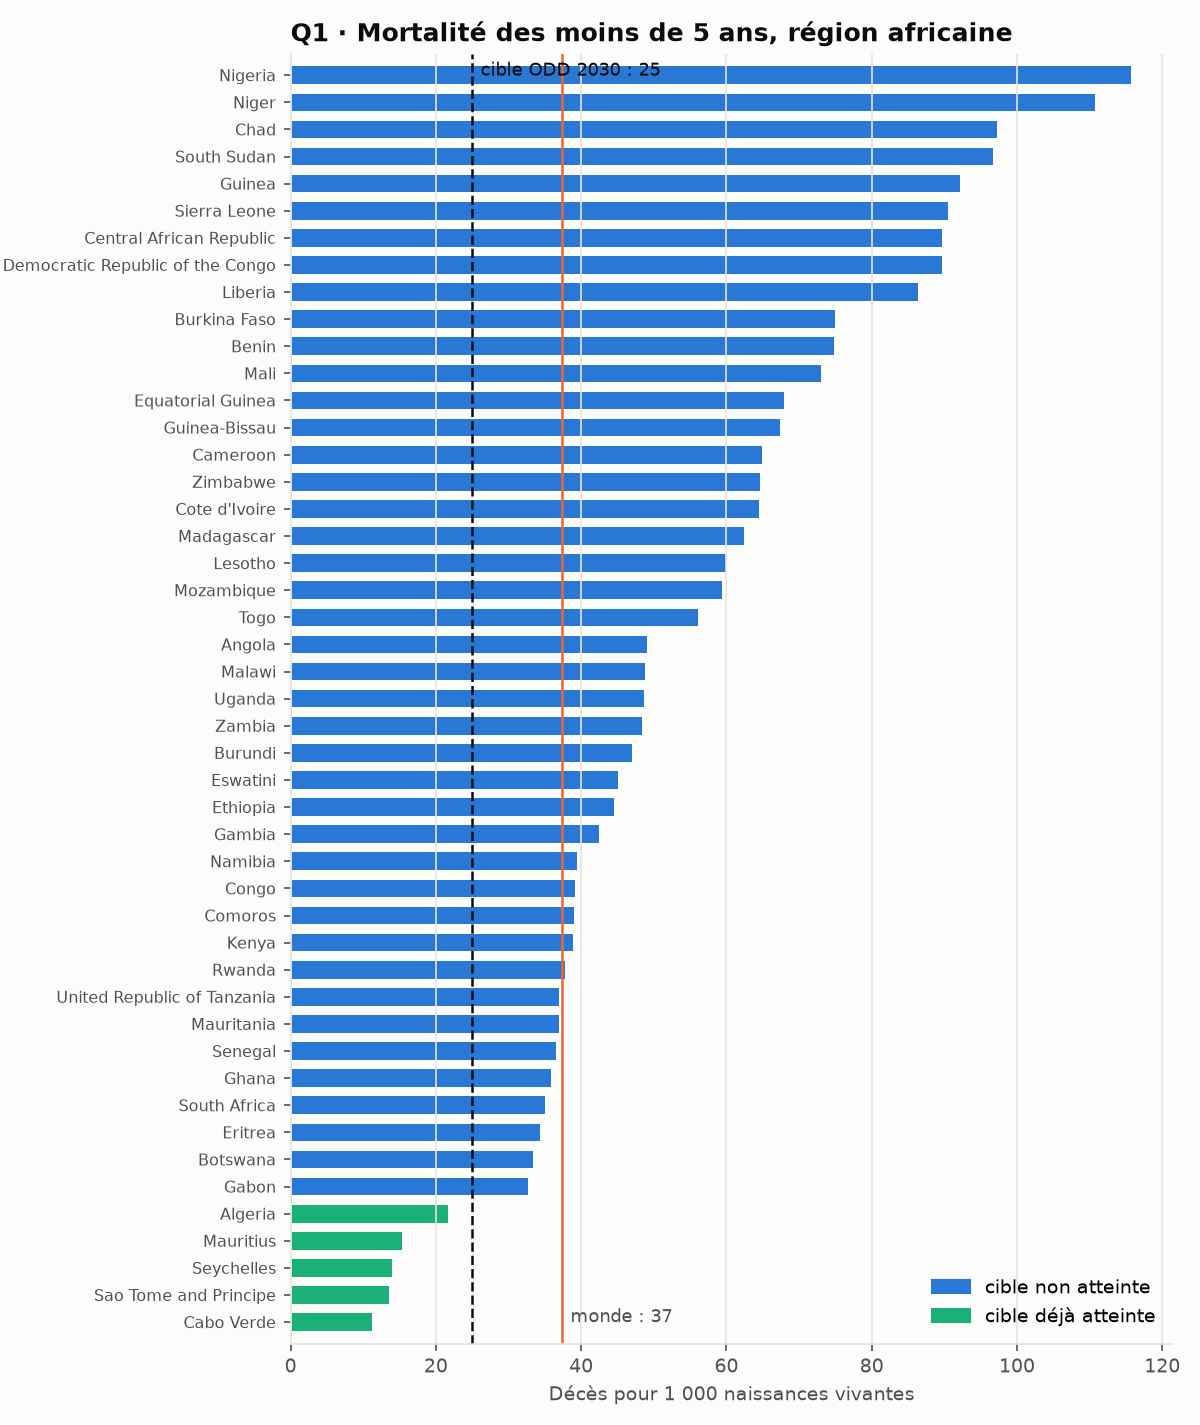
\includegraphics[width=0.78\linewidth]{q1_mortalite_moins_5_ans.png}
\caption{Mortalité des moins de 5 ans par pays de la région africaine (2024)}
\end{figure}

\begin{figure}[H]
\centering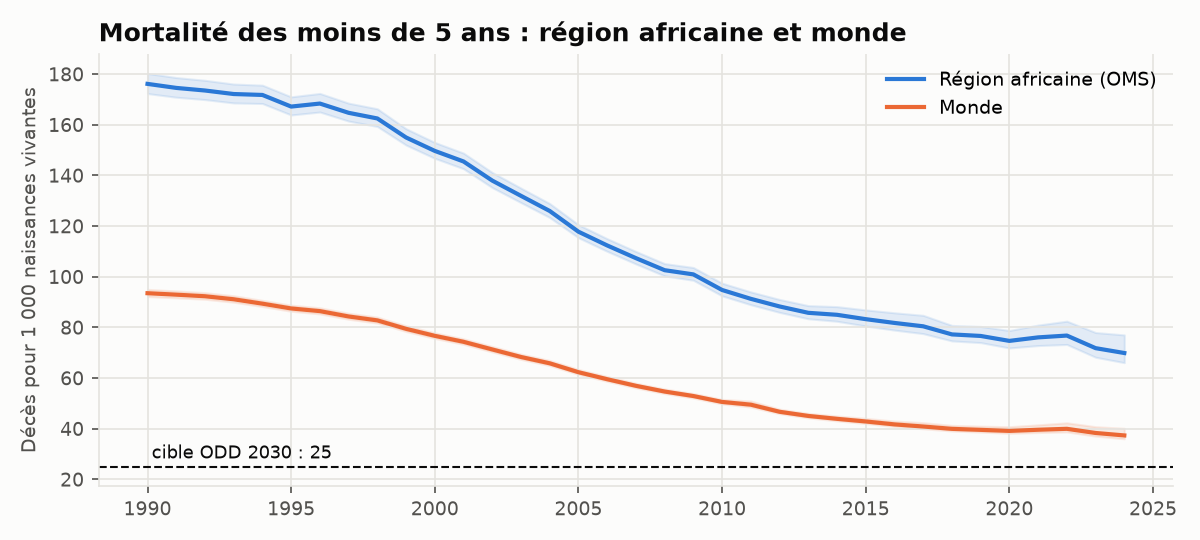
\includegraphics[width=0.92\linewidth]{q1_tendance_region_monde.png}
\caption{Évolution depuis 1990, avec intervalles d'incertitude}
\end{figure}

La mortalité des moins de 5 ans de la région a été divisée par 2,5 depuis 1990, de 176 à 70~‰. Elle reste près de deux fois supérieure à
la moyenne mondiale. La valeur régionale (70~‰) dépasse nettement la médiane des pays (48,7~‰) : les pays les plus peuplés, comme le Nigeria
(116~‰), pèsent lourd dans le total régional.

\subsection{Q2 · Quels pays atteindront les cibles d'ici 2030 ?}
Méthode du \textbf{taux annuel moyen de réduction} (ARR), utilisée par le groupe interagences des Nations unies pour l'estimation de la mortalité
de l'enfant : $\text{ARR} = \ln(v_{2015} / v_{t}) / (t - 2015)$, puis projection à 2030 en supposant que ce rythme se maintient.

\begin{figure}[H]
\centering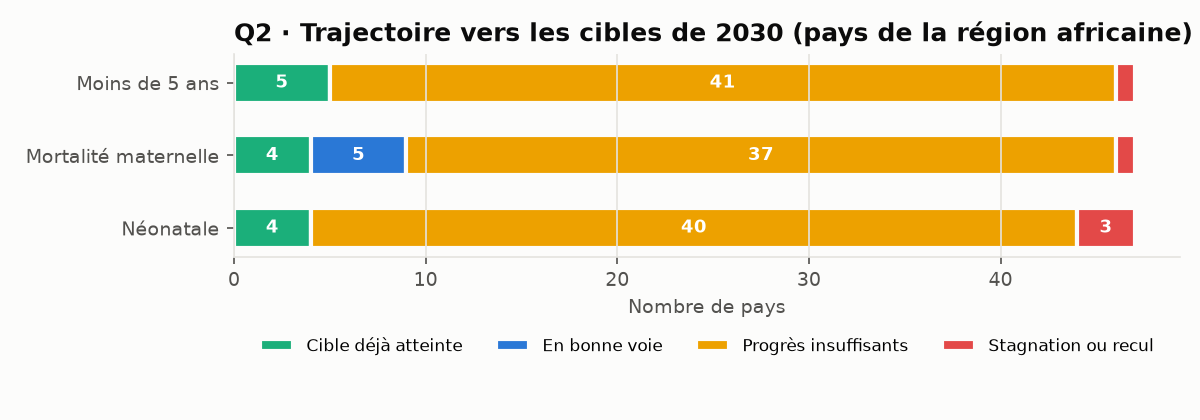
\includegraphics[width=0.92\linewidth]{q2_trajectoires_2030.png}
\caption{Statut des pays de la région africaine par rapport à leur trajectoire}
\end{figure}

\begin{itemize}[leftmargin=1.2em]
  \item \textbf{Mortalité des moins de 5 ans :} aucun pays hors cible n'est en bonne voie. Le pays médian réduit sa mortalité de \textbf{3,0~\% par an}
        alors qu'il faudrait \textbf{12,4~\%}. Le Zimbabwe recule (59,2 → 64,7~‰ depuis 2015).
  \item \textbf{Mortalité maternelle :} c'est la seule cible où 5 pays sont en bonne voie : Eswatini, Mozambique, Namibie, Sao Tomé-et-Principe
        et Zambie, avec des réductions de 7 à 11~\% par an. Le Botswana recule.
  \item \textbf{Mortalité néonatale :} la plus lente (1,7~\% par an). Elle stagne ou recule au Nigeria, en Afrique du Sud et au Zimbabwe.
\end{itemize}

\subsection{Q3 · Quel écart entre les ménages les plus pauvres et les plus riches ?}
\begin{figure}[H]
\centering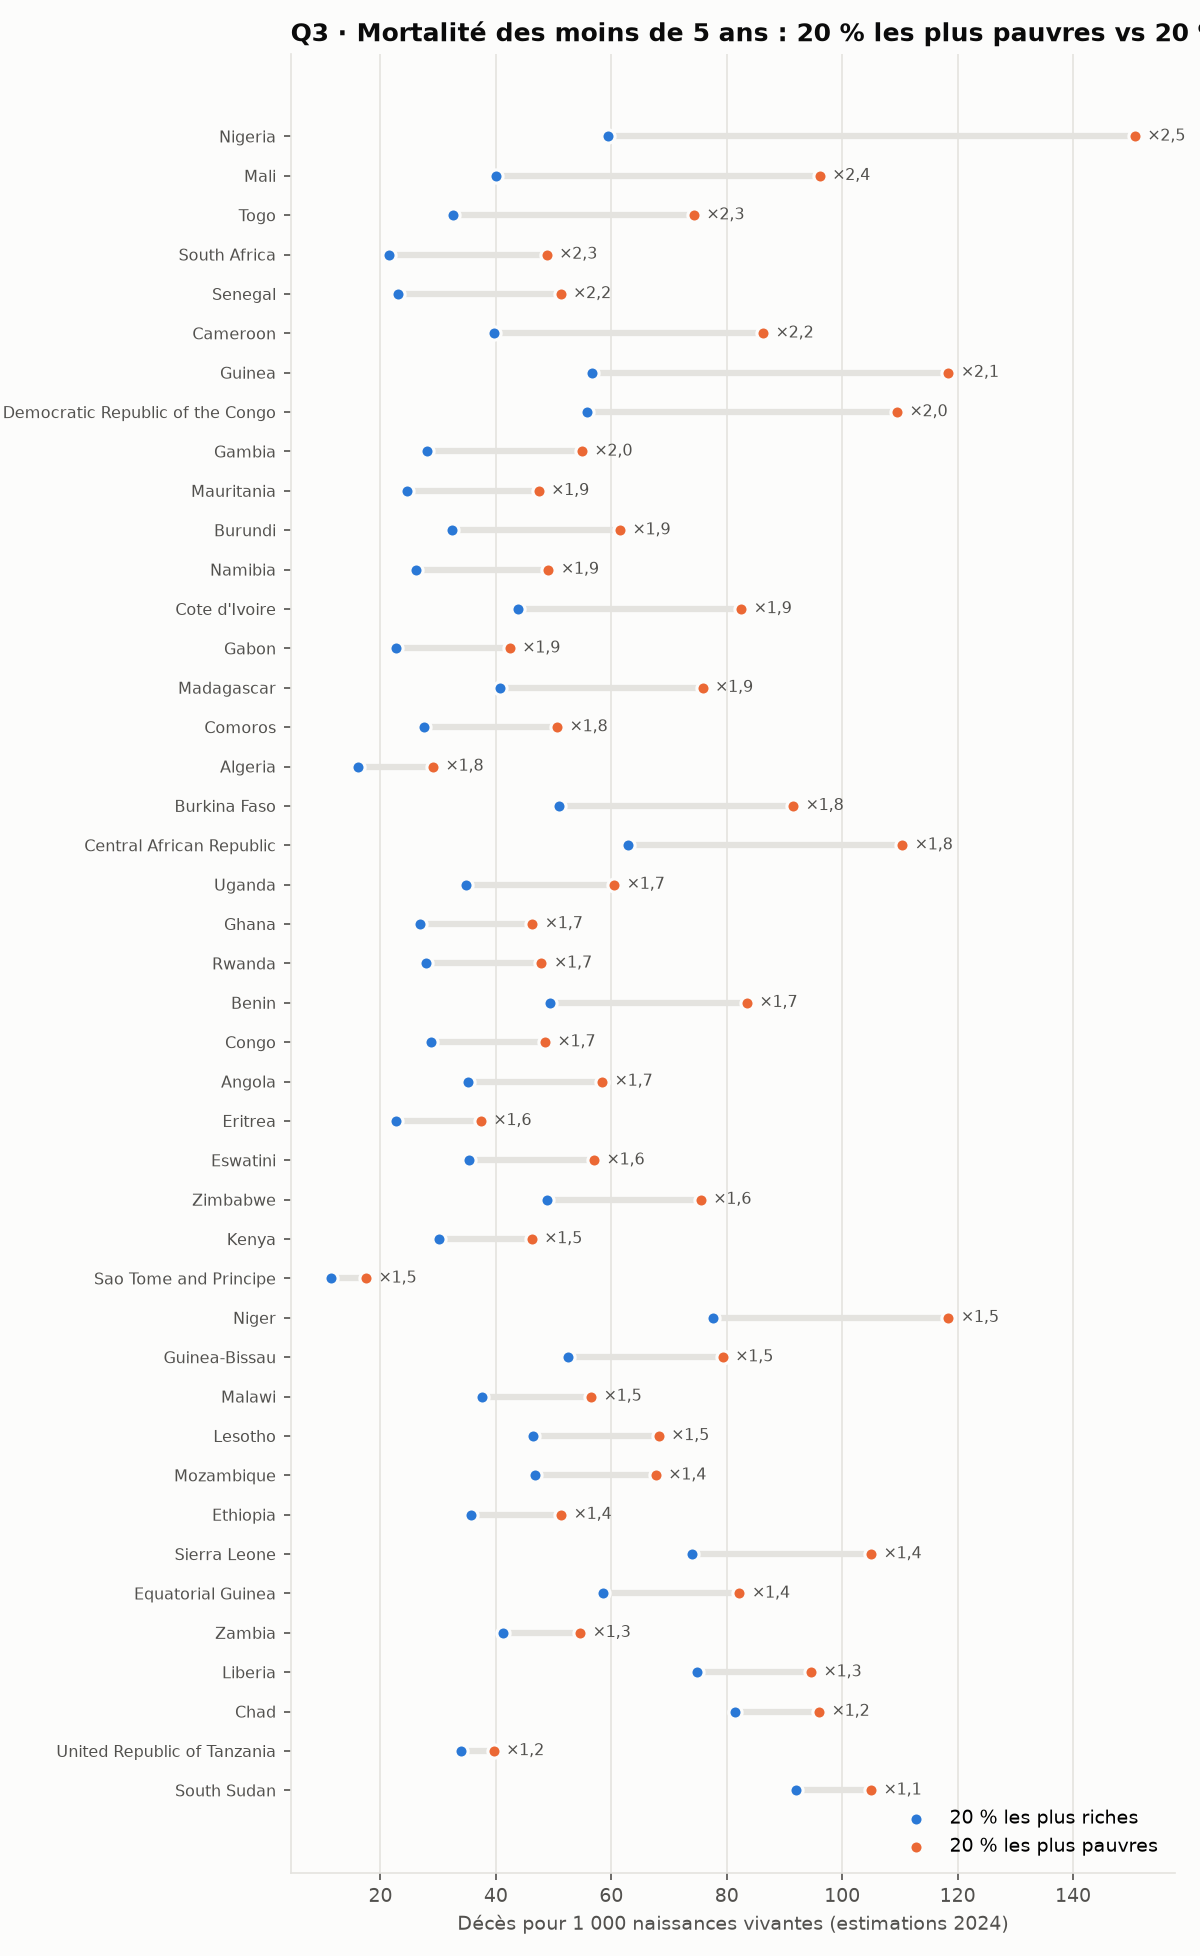
\includegraphics[width=0.74\linewidth]{q3_inegalites_richesse.png}
\caption{Mortalité des moins de 5 ans : 20~\% les plus pauvres contre 20~\% les plus riches (2024)}
\end{figure}

\begin{table}[H]
\centering\small
\begin{tabularx}{\linewidth}{@{}l r r r r@{}}
\toprule
\textbf{Année} & \textbf{20~\% les plus pauvres} & \textbf{20~\% les plus riches} & \textbf{Écart absolu} & \textbf{Ratio} \\
\midrule
1990 & 186,6 & 118,8 & 63,3 & 1,56 \\
2000 & 159,7 & 94,2 & 50,5 & 1,49 \\
2015 & 74,4 & 46,3 & 28,2 & 1,67 \\
2024 & 61,5 & 37,6 & 23,2 & 1,71 \\
\bottomrule
\end{tabularx}
\caption{Valeurs médianes de 43 pays de la région africaine (décès pour 1\,000 naissances vivantes)}
\end{table}

Un enfant né dans les 20~\% de ménages les plus pauvres a \textbf{1,7 fois plus de risque} de mourir avant 5 ans, et jusqu'à 2,5 fois au Nigeria
et 2,4 fois au Mali. \textbf{L'écart absolu s'est réduit} de 63 à 23~‰, mais \textbf{l'écart relatif se creuse depuis 2000} : les ménages
aisés progressent proportionnellement plus vite.

\subsection{Q4 · Les moyens vont-ils de pair avec les résultats ?}
\begin{figure}[H]
\centering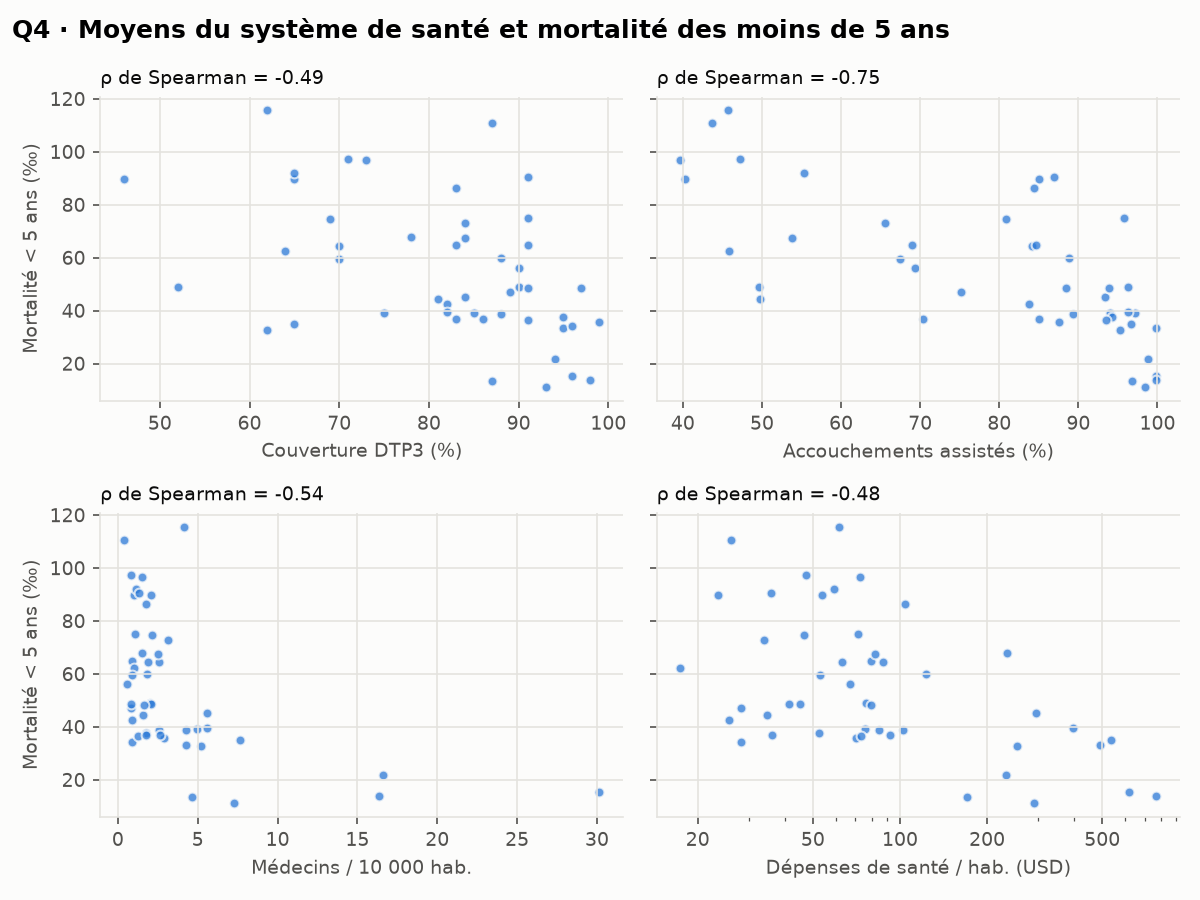
\includegraphics[width=0.86\linewidth]{q4_moyens_resultats.png}
\caption{Indicateurs de moyens et mortalité des moins de 5 ans (un point = un pays)}
\end{figure}

Tous les moyens sont associés à une mortalité plus faible, mais avec une intensité très différente : \textbf{accouchements assistés}
($\rho = -0{,}75$, sur 45 pays), médecins ($-0{,}54$), vaccination DTP3 ($-0{,}49$), dépenses de santé ($-0{,}48$). Il s'agit de
\textbf{corrélations}, pas de preuves de causalité : ces moyens reflètent aussi le niveau de développement général des pays.

\subsection{Recommandations au conseil d'administration}
\begin{keybox}[Pour Initiative Baobab Santé]
\begin{enumerate}[leftmargin=1.4em]
  \item \textbf{Prioriser la mortalité néonatale :} c'est la cible qui progresse le plus lentement (1,7~\% par an). Les décès du premier mois
        représentent près de la moitié de la mortalité des moins de 5 ans (médianes : 23,0 sur 48,7~‰).
  \item \textbf{Cibler explicitement les ménages pauvres :} l'écart relatif se creuse. Un programme non ciblé profite d'abord aux ménages aisés.
  \item \textbf{Miser sur l'accouchement assisté :} c'est le levier le plus fortement associé à une faible mortalité dans la région.
  \item \textbf{Étudier les pays en bonne voie} sur la mortalité maternelle (Mozambique, Zambie, Eswatini…) pour en tirer des enseignements.
  \item \textbf{Relancer le pipeline après chaque publication de l'OMS :} les révisions sont désormais intégrées et tracées automatiquement.
\end{enumerate}
\end{keybox}

% =============================================================================
\section{Limites et dette technique}\label{sec:limites}

\begin{tabularx}{\linewidth}{@{}L{5.4cm} Y@{}}
\toprule
\textbf{Limite} & \textbf{Conséquence} \\
\midrule
Les données de l'OMS sont des estimations modélisées & Les intervalles d'incertitude sont stockés, mais pas encore affichés pour chaque pays \\
Projection linéaire du rythme (ARR) & Elle suppose que le rythme 2015-2024 se maintient jusqu'en 2030 \\
Corrélations (Q4) & Elles ne prouvent aucune causalité \\
Noms de pays en anglais & L'API de l'OMS ne publie pas de libellés français \\
\midrule
\multicolumn{2}{@{}l}{\textbf{Dette technique assumée au niveau 1}} \\
\midrule
Seule la dernière valeur est conservée & L'historique complet des révisions sera introduit au projet 2 \\
Suppressions de l'OMS non gérées & Une observation retirée par l'OMS resterait en base \\
Pas de planification & Exécution manuelle (orchestration au projet 3) \\
Pas d'intégration continue & Les tests sont lancés à la main (CI/CD au projet 3) \\
\bottomrule
\end{tabularx}

% =============================================================================
\section{Retour d'expérience}
\begin{itemize}[leftmargin=1.2em]
  \item \textbf{Le grain d'abord :} 8 valeurs « identiques » cachaient une dimension. Comprendre le grain avant de modéliser évite l'erreur du client.
  \item \textbf{Un contrôle de qualité se calibre :} 25 valeurs « aberrantes » étaient des catastrophes historiques réelles.
  \item \textbf{Mesurer au lieu de supposer :} 130~s perdues dans une résolution DNS, pas dans le code.
  \item \textbf{Les tests trouvent de vrais bugs :} le piège \texttt{None} / \texttt{NaN} aurait vidé la base en production.
  \item \textbf{Vérifier ses propres hypothèses :} les données par richesse n'étaient pas issues d'enquêtes ponctuelles, et cette vérification
        a ouvert la question de l'évolution des inégalités.
\end{itemize}

% =============================================================================
\section{Feuille de route}
\begin{tabularx}{\linewidth}{@{}L{4.6cm} Y@{}}
\toprule
\textbf{Évolution} & \textbf{Apport} \\
\midrule
Historisation des révisions & Table d'historique (\emph{slowly changing dimension} de type 2), au programme du projet 2 \\
Chargement incrémental & Ne télécharger que les indicateurs mis à jour (champ \texttt{Date} de l'OMS) \\
Orchestration et CI/CD & Exécution planifiée après chaque publication, tests automatiques à chaque modification (projet 3) \\
Tableau de bord & Visualisation interactive pour l'équipe du client, connectée directement à PostgreSQL \\
\bottomrule
\end{tabularx}

% =============================================================================
\appendix
\section{Requêtes SQL livrées}
\begin{tabularx}{\linewidth}{@{}L{5.2cm} Y@{}}
\toprule
\texttt{00\_schema.sql}, \texttt{01\_views.sql} & Schéma (idempotent) et vues d'analyse \\
\texttt{q0\_couverture\_donnees.sql} & Couverture des données dans la région \\
\texttt{q1\_cibles\_2030.sql} & Situation par rapport aux cibles \\
\texttt{q2\_rythme\_2030.sql}, \texttt{q2b\_…} & Trajectoire par pays et synthèse (méthode ARR) \\
\texttt{q3\_inegalites\_richesse.sql}, \texttt{q3b\_…} & Écart pauvres / riches, et son évolution depuis 1990 \\
\texttt{q4\_moyens\_resultats.sql} & Corrélations entre moyens et mortalité \\
\texttt{controle\_recette.sql} & Contrôles de recette (C2, C3, C4) \\
\bottomrule
\end{tabularx}

\section{Décisions d'architecture (ADR)}
\begin{tabularx}{\linewidth}{@{}l Y@{}}
\toprule
ADR 001 & PostgreSQL conteneurisé avec Docker Compose, secrets dans \texttt{.env} \\
ADR 002 & Chargement par staging et UPSERT, clé métier complète \texttt{NULLS NOT DISTINCT} \\
ADR 003 & Contrôles de qualité, quarantaine et calibrage des seuils \\
\bottomrule
\end{tabularx}

\section{Glossaire}
\begin{tabularx}{\linewidth}{@{}>{\bfseries}L{3.6cm} Y@{}}
ODD 3 & Objectif de développement durable n°3 des Nations unies : « Bonne santé et bien-être » \\
Grain & Ce que représente une ligne d'une table \\
Staging & Zone de transit où le lot est chargé avant d'être fusionné dans les tables de référence \\
UPSERT & Insérer si la ligne est nouvelle, mettre à jour si elle existe (\emph{update} + \emph{insert}) \\
Quarantaine & Table qui conserve les lignes refusées par les contrôles, avec leur motif \\
ARR & \emph{Annual Rate of Reduction} : taux annuel moyen de réduction d'un indicateur \\
Quintile de richesse & Cinquième de la population classée selon la richesse du ménage (Q1 : 20~\% les plus pauvres) \\
Conteneur & Environnement isolé et reproductible qui exécute un logiciel, ici PostgreSQL \\
\end{tabularx}

\end{document}
